\documentclass[14pt]{matmex-diploma-custom}
\usepackage{listings}
\usepackage{amsmath}
\usepackage{amssymb}
\usepackage{amsthm}
\usepackage{float}
\usepackage[caption=false]{subfig}
\usepackage{minted}
\usepackage{verbments}
\usepackage{caption}
%\usepackage{algorithmicx}
\usepackage{tikz} 
\usepackage{pgfplots} 
\usepackage{sidecap} 
\usepackage{soul}
\usepackage{xcolor}
\usepackage{multirow}
%\usepackage{tabu}
%\usepackage{float}

% Package to generate and customize Algorithm as per ACM style
\usepackage[ruled, linesnumbered]{algorithm2e}
\renewcommand{\algorithmcfname}{Алгоритм}
\SetAlFnt{\small}
\SetAlCapFnt{\small} 
\SetAlCapNameFnt{\small}
\SetAlCapHSkip{0pt}
\IncMargin{-\parindent}

%\documentclass[14pt]{matmex-diploma-custom}
%\hyphenation{Ge-ne-ra-lised}
\newtheorem{mydef}{Определение}
%\tolerance=1
\emergencystretch=\maxdimen
%\hyphenpenalty=10000
%\hbadness=10000
\usetikzlibrary{graphs, graphs.standard, quotes}
\usetikzlibrary{arrows}

\renewcommand{\lstlistingname}{Листинг}
\renewcommand\listingscaption{Листинг}


\begin{document}


\makeatletter
\let\@upn\textbf% \textup -> \textbf
\makeatother
\newtheorem{theorem}{Теорема}
\newtheorem{lemma}{Лемма}


% Год, город, название университета и факультета предопределены,
% но можно и поменять.
% Если англоязычная титульная страница не нужна, то ее можно просто удалить.
\filltitle{ru}{
	chair              = {Математическое обеспечение и администрирование\\ информационных систем\\
		\vskip 1em
		Системное программирование},
	title              = {Оптимизация алгоритмов синтаксического анализа, основанных на матричных операциях},
	% Здесь указывается тип работы. Возможные значения:
	%   coursework - Курсовая работа
	%   diploma - Диплом специалиста
	%   master - Диплом магистра
	%   bachelor - Диплом бакалавра
	type               = {diploma},
	position           = {студента},
	group              = 444,
	author             = {Сусанина Юлия Алексеевна},
	supervisorPosition = {к.\,ф.-м.\,н., доцент},
	supervisor         = {Григорьев С.\,В.},
	reviewerPosition   = {научный координатор Центра Компьютерных Наук TUCS},
	reviewer           = {Бараш М.\,Л.},
	%chairHeadPosition  = {д.\,ф.-м.\,н., профессор},
	%chairHead          = {Терехов А.\,Н.}
}
\filltitle{en}{
    chair = {Software and Administration of Information Systems \\ \vspace{5mm} Software Engineering},
    title = {Optimization of parsing by matrix multiplication},
    type = {diploma},
    author = {Yulia Susanina},
    supervisorPosition = {Assistant Professor},
    supervisor = {Semyon Grigorev},
    reviewerPosition = {Ph.D., Scientific Coordinator, Turku Center for Computer Science},
    reviewer = {Mikhail Barash},
    %chairHeadPosition = {Professor},
    %chairHead = {Andrey Terekhov},
    }

\maketitle
%\setcounter{tocdepth}{1}
\tableofcontents
% У введения нет номера главы
\section*{Введение}

Теория формальных языков активно изучается и находит широкое применение во многих областях, прежде всего, для описания языков программирования и естественных языков. 
Также существует множество исследований, которые показывают эффективность использования формальных языков в биоинформатике  для решения задач распознавания и классификации, некоторые из которых основаны на том, что вторичная структура геномных последовательностей содержит в себе важную информацию об организме. 
Характерные особенности вторичной структуры могут быть описаны с помощью некоторой контекстно-свободной (КС) грамматики, что позволяет свести проблему распознавания и классификации к задаче синтаксического анализа (определения принадлежности некоторой строки к языку, заданному грамматикой)~\cite{knudsen1999rna, dowell2004evaluation, rivas2000language}. 
Часто необходимо не просто проверить выводимость конкретной строки, но и найти все подстроки, принадлежащие некоторому формальному языку~\cite{durbin1996biological}.

Большинство подходов к анализу биологических цепочек, которые основаны на синтаксическом анализе, сталкиваются с одной и той же проблемой: низкая производительность. 
Чаще всего в них применяется алгоритм CYK~\cite{kasami1966efficient, Younger:1966:CLP:1441427.1442019}, который работает за кубическое время и неэффективен на длинных строках и для больших грамматик~\cite{liu2005parallel}. 
Необходимым требованием таких областей применения, как биоинформатика, является обработка больших объёмов данных, что приводит к необходимости усовершенствования существующих методов синтаксического анализа.
Более того, некоторые особенности вторичной структуры не могут быть выражены с помощью КС-грамматик и требуют применения других классов грамматик~\cite{zier2013rna}.

На данный момент одним из самых быстрых алгоритмов, работающих с любой КС-грамматикой, является алгоритм Валианта~\cite{Valiant:1975:GCR:1739932.1740048}. 
Также данный алгоритм можно легко расширить для конъюнктивных и булевых грамматик, которые обладают большей выразительностью~\cite{Okhotin:2014:PMM:2565359.2565379}. 
Однако в связи с сложностью  применения к выше упомянутой задаче поиска всех подстрок и отсутсвия эффективной реализации алгоритм Валианта достаточно редко используется на практике, несмотря на широкие теоретические возможности.

В лаборатории языковых инструментов Jetbrains, СПбГУ~\cite{jetbrains}, Анной Явейн был предложен алгоритм, являющийся модификацией алгоритма Валианта~\cite{alg} и обладающий определенными преимуществами, такими как легкость адаптации к задаче поиска подстрок и возможность повысить использование GPGPU и параллельных вычислений.



\section{Постановка задачи}

Целью данной работы является исследование алгоритма Явейн, являющегося модификацией алгоритма Валианта.
Для её достижения были поставлены следующие задачи.

\begin{itemize}
	\item Изучить алгоритм Явейн.
	\item Доказать корректность алгоритма Явейн и дать оценку сложности.
	\item Проанализировать эффективность применения этого алгоритма и алгоритма Валианта к задаче поиска подстрок.
	\item Реализовать последовательную и параллельную версии алгоритмов Валианта и Явейн.
	\item Экспериментальное исследование алгоритма Явейн.
\end{itemize}
	

\section{Обзор}

В данном разделе мы введем основные определения из теории формальных языков и опишем алгоритмы синтаксического анализа, рассматриваемые в данной работе: алгоритмы Валианта и Явейн. Также мы отметим области применения данных алгоритмов и остановимся на биоинформатике, в частности, задаче поиска подстрок.

\subsection{Терминология}

Алфавитом $\Sigma$ будем называть некоторое конечное множество символов.
$\Sigma^{*}$ --- это множество всех конечных строк над алфавитом $\Sigma$.

Контекстно-свободная (КС) грамматика --- четверка $(\Sigma, N, R, S)$, где $\Sigma$ --- конечное множетство терминальных символов, $N$ --- конечное множество нетерминальных символов, $R$ --- конечное множество правил вида $A \rightarrow \beta$, где $A \in N$, $\beta \in V^{*}$, $V = \Sigma \cup N$ и $S \in N$ --- стартовый символ.

КС-грамматика $G_S = (\Sigma, N, R, S)$ называется грамматикой в нормальной форме Хомского, если все ее правила имеют одну из следующих форм: $A \rightarrow BC$, $A \rightarrow a$, или $S \rightarrow \varepsilon$, 
где $A, B, C \in N, a \in \Sigma$ и $\varepsilon$ --- пустая строка.

$L_{G}(A) = \{ \omega | A\xrightarrow{*} \omega\}$ --- язык, порождаемый грамматикой $G_{A} = (\Sigma, N, R, A)$, где $A \xrightarrow{*} \omega$ означает, что $\omega$ может быть получена из нетерминала $A$ путем применения некотороый последовательности правил из $R$.

\subsection{Алгоритм Валианта}

Основной задачей синтаксического анализа является определение принадлежности некоторой строки языку, заданному грамматикой.

Алгоритм Валианта относится к табличным методам синтаксического анализа, которым на вход обычно подается грамматика в нормальной форме Хомского $G_S = (\Sigma, N, R, S)$ и некоторая строка $a_{1} \dots a_{n}$, где $n + 1$ --- степень двойки. Результатом работы данного алгоритма является верхнетреугольная матрица разбора $T$, элементами которой являются подмножества нетерминалов. Каждый элемент отвечает за вывод конкретной подстроки: $T_{i, j} =  \{ A | A \in N, a_{i + 1} \dots a_{j} \in L_{G}(A)\} \quad \forall i < j$.

Элементы инициализируются пустыми множествами.
Сначала заполняется диагональ: $T_{i - 1, i} = \{ A | A \rightarrow a_{i} \in R\}.$ 
Затем, матрица начинает последовательно заполняться по формуле:
$T_{i, j} = f(P_{i, j}),$ 
где $P_{i, j} = \bigcup\limits_{k = i + 1}^{j - 1} T_{i,k} \times T_{k, j}$ и
$f(P_{i, j}) = \{A | \exists A \rightarrow BC \in R : (B, C) \in P_{i, j}\}.$

Входная строка $a_{1}a_{2} \dots a_{n}$ принадлежит языку $L_{G}(S)$ тогда и только тогда, когда $S \in T_{0, n}$.

Если все элементы данной матрицы заполнять последовательно, то вычислительная сложность данного алгоритма будет составлять $O(n^3)$. Валиант немного изменил порядок вычисления элементов, за счет чего смог свести самую затратную по времени операцию $\bigcup\limits_{k = i + 1}^{j - 1} T_{i, k} \times T_{k, j}$ к задаче умножения некоторого количества булевых матриц.

Определим перемножение двух подматриц матрицы разбора $T$ следующим образом: пусть $X \in (2^N)^{m \times l}$ и $Y \in (2^N)^{l \times n}$ --- подматрицы $T$, тогда $X \times Y = Z$, где $Z \in (2^{N \times N})^{m \times n}$ и $Z_{i, j} = \bigcup\limits_{k = 1}^{l} X_{i, k} \times Y_{k, j}$.

Теперь можно представить вычисление $X \times Y$ как перемножение $|N|^2$ булевых матриц (для каждой пары нетерминалов).
Определим матрицу, соответствующую паре $(B, C) \in N \times N$, как $Z^{(B, C)}$, тогда $Z_{i, j}^{(B, C)} = 1$ тогда и только тогда, когда $(B, C) \in Z_{i, j}$.
Заметим также, что $Z^{(B, C)} = X^{B} \times Y^{C}$.
Каждое такое перемножение может совершаться абсолютно независимо.
С этими изменениями сложность алгоритма будет составлять $\mathcal{O}(|G|BMM(n)log(n))$ для строки длины $n$, где $BMM(n)$ --- количество операций, необходимое для перемножения двух булевых матриц размера $n \times n$.

Опишем алгоритм Валинта более подробно (Алгоритм 1). 
Все элементы матриц $T$ и $P$ заполняются с помощью двух рекурсивных процедур.
Процедура $compute(l, m)$ корректно заполняет $T_{i,j}$ для всех $l \le i < j < m$.
Процедура $complete(l, m, l', m')$ вычисляет $T_{i, j}$ для всех $l \le i < m$, $l' \le j < m'$. Предполагается, что $T_{i, j}$ для всех $l \leq i < j < m,  l' \leq i < j < m'$ уже корректно заполнены и $P_{i, j} =  \{ (B, C) |\exists k, (m \le k < l'), a_{i + 1} \dots a_{k} \in L(B), a_{k + 1} \dots a_{j} \in L(C)\}$ для всех $l \leq i < m,  l' \leq j < m'$.

% Algorithm1
\begin{algorithm}[h]
\SetAlgoNoLine
\KwIn{Грамматика $G = (\Sigma, N, R, S), w = a_{1} \dots a_{n}, n \geq 1, a_{i} \in \Sigma$, где  $n + 1 = 2^k$}
\underline{main()}{:}{

 \textit{compute(0, n + 1)\;}
 accept if and only if $S \in T_{0, n}$
 \linebreak
 }

\underline{compute(\textit{l, m})}{:}{

 \If {$m - l \geq 4$}{
     \textit{compute(l, $\frac{l+m}{2}$)\;
     compute($\frac{l+m}{2}$, m)}}
 \textit{complete(l, $\frac{l+m}{2}$, $\frac{l+m}{2}$, m)}
 \linebreak
 }

\underline{complete(\textit{l, m}, $l^\prime$, $m^\prime$)}{:}{

 \lIf {$m - l = 4$ and $m = l^\prime$}{$T_{l, l + 1} = \{A | A \rightarrow a_{l+ 1} \in R\}$}
 \lElseIf{$m - l = 1$ and $m < l^\prime$}{ $T_{l, l'} = f(P_{l, l'})$}
 \ElseIf{$m - l > 1$}{
    $\textit{leftgrounded} = (l, \frac{l+m}{2}, \frac{l+m}{2}, m), \textit{rightgrounded} = (l', \frac{l'+m'}{2}, \frac{l'+m'}{2}, m')$,

    $\textit{bottom} = (\frac{l+m}{2}, m, l', \frac{l'+m'}{2}), left = (l, \frac{l+m}{2}, l', \frac{l'+m'}{2})$,

    $\textit{right} = (\frac{l+m}{2}, m, \frac{l'+m'}{2}, m'), top = (l, \frac{l+m}{2}, \frac{l'+m'}{2}, m')$\;
    \textit{complete(bottom)}\;
    $P_{\textit{left}} = P_{\textit{left}} \cup (T_{\textit{leftgrounded}} \times T_{\textit{bottom}})$\;
    \textit{complete(left)}\;
    $P_{\textit{right}} = P_{\textit{right}} \cup (T_{\textit{bottom}} \times T_{\textit{rightgrounded}})$\;
    \textit{complete(right)}\;
    $P_{\textit{top}} = P_{\textit{top}} \cup (T_{\textit{leftgrounded}} \times T_{\textit{right}})$\;
    $P_{\textit{top}} = P_{\textit{top}} \cup (T_{\textit{left}} \times T_{\textit{rightgrounded}})$\;
    \textit{complete(top)}
    }
 }
\caption{Алгоритм Валианта}
\label{algo:valiant}
\end{algorithm}

\subsection{Алгоритм Явейн}

Теперь рассмотрим алгоритм, являющийся модификацией алгоритма Валианта. Его главным отличием является возможность разбиения матрицы разбора на слои непересекающихся подматриц.

Заполнение слоев происходит последовательно, снизу вверх. Слой состоит из квадратных подматриц размера $2^n$, $n > 0$. На момент начала заполнения слоя нижняя часть матриц ($bottom$) уже заполнена, так как принадлежит предыдущему слою, поэтому эти слои мы также будем называть V-образными. Пример разбиения матрицы разбора на слои показан на рис.~\ref{fig2}. Заметим, что каждую матрицу слоя можно обрабатывать параллельно. 


\begin{figure}
\vspace{3mm}
 \begin{center}
    \centering
    
\includegraphics[width=10cm]{layers.png}
    \caption{Деление матриц на V-образные слои}
    \label{fig2}
 \end{center}
\vspace{-8mm}
\end{figure}

Пример работы алгоритма показан на рис.~\ref{modvis}. Нижний слой, состоящий из подматриц размера 1, вычисляется заранее, а заполнение матрицы начинается со второго слоя. (Здесь и далее, под слоем матриц будем понимать некоторое множество её подматриц разбора.) Более того, на рис. 4 на каждом шаге изображены операции, которые могут быть выполненные независимо, что позволяет значительно упростить разработку параллельной версии алгоритма.

\begin{figure}[h]
\vspace{3mm}
 \begin{center}
    \centering
    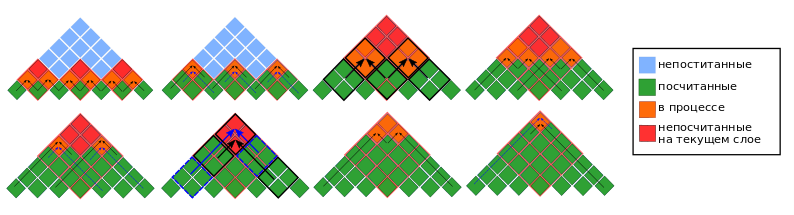
\includegraphics[width=16cm]{modivis2.png}
    \caption{Деление матриц на V-образные слои}
    \label{modvis}
 \end{center}
\vspace{-8mm}
\end{figure}

Функция \textit{main()} (Алгоритм 2) заполняет диагональ:  $(T_{l, l+1})$, затем делит матрицу на слои и вычисляет их с помощью процедуры \textit{completeVLayer()}.

Дополнительные функции \textit{left(subm)}, \textit{right(subm)}, \textit{top(subm)}, \textit{bottom(subm)}, \textit{rightgrounded(subm)} and \textit{leftgrounded(subm)} возвращают подматрицы матрицы $\textit{subm} = (l, m, l', m')$ аналогично алгоритму~\ref{algo:valiant}.

Процедура \textit{completeVLayer(M)} на вход принимает слой (массив подматриц)  $M$ и для каждой \textit{subm = (l, m, l', m') $\in M$} заполняет \textit{left(subm), right(subm), top(subm)}.
Предполагается, что \textit{bottom(subm)} и $T_{i, j}$ для всех $i$, $j$, таких что $l \leq i < j < m$, $  l' \leq i < j < m'$ уже корректно вычислены и 
$P_{i, j} =  \{ (B, C) | \exists k, (m \le k < l'), a_{i + 1} \dots a_{k} \in L_G(B), a_{k + 1} \dots a_{j} \in L_G(C)\} $ для всех $i$, $j$, таких что $l \leq i < m$, $l' \leq j < m'$.


\begin{algorithm}[!h]
\SetAlgoNoLine
\KwIn{Грамматика $G = (\Sigma, N, R, S), w = a_{1} \dots a_{n}, n \geq 1, a_{i} \in \Sigma$, где  $n + 1 = 2^p$}
\underline{main()}{:}{

 \lFor {$l \in \{1, \ldots, n \}$}{$T_{l, l + 1} = \{A | A \rightarrow a_{l + 1} \in R\}$}
 \For{$1 \le i < p - 1 $}{
 \textit{layer = constructLayer($i$)}\;
 \textit{completeVLayer(layer)}
 }
 accept if and only if $S \in T_{0, n}$
 \BlankLine
 }

\underline{constructLayer(i)}{:}{
 \BlankLine
 $\{(k2^i, (k+1)2^i, (k + 1)2^i, (k+2)2^i) \, |\, 0 \le k < 2^{p - i} - 1\}$
 \BlankLine
    }
\underline{completeLayer(M)}{:}{
\BlankLine
\If {$\forall (l, m, l', m') \in M \quad (m - l = 1)$}{\lFor{$ (l, m, l', m') \in M$}{$T_{l, l'} = f(P_{l, l'})$}}
\Else{
\textit{completeLayer($\{\textit{bottom(subm)}\, |\,\textit{subm} \in M \})$}\;
\textit{completeVLayer(M)}
}
\BlankLine
}

\underline{completeVLayer(M)}{:}{
 \BlankLine
 $\textit{multiplicationTasks}_1 = \linebreak
    \{\textit{left(subm)}, \textit{leftgrounded(subm)}, \textit{bottom(subm)}\, 
    |\,\textit{subm} \in M \} \cup \linebreak  \{\textit{right(subm)}, \textit{bottom(subm)}, \textit{rightgrounded(subm)}\, |\,\textit{subm} \in M\}$\;
 \BlankLine
 \textit{multiplicationTask$_2$} = $\{\textit{top(subm)}, \textit{leftgrounded(subm)}, \textit{right(subm)}\, |\,\textit{subm} \in M\}$\;
 \BlankLine
 \textit{multiplicationTask$_3$} = $\{\textit{top(subm)}, \textit{left(subm)}, \textit{rightgrounded(subm)}\, |\,\textit{subm} \in M\}$\;
 \BlankLine
 \textit{performMultiplications(multiplicationTask$_1$)}\;
 \textit{completeLayer($\{\textit{left(subm)}\, |\,subm \in M \} \cup \{\textit{right(subm)}\, |\,\textit{subm} \in M \}$)}\;
 \textit{performMultiplications(multiplicationTask$_2$)}\;
 \textit{performMultiplications(multiplicationTask$_3$)}\;
 \textit{completeLayer($\{top(subm)\, |\,subm \in M \}$)}

 }
 \BlankLine

 \underline{performMultiplication(tasks)}{:}{\\
 \lFor{$ (m, m1, m2) \in \textit{tasks}$}{$P_{m} = P_{m} \cup (T_{m1} \times T_{m2})$}
 }

\caption{Алгоритм Явейн}
\label{algo:modified}
\end{algorithm}

Процедура \textit{completeLayer(M)} также принимает массив матриц $M$, но заполняет $T_{i, j}$ для всех $(i, j) \in subm$.
Ограничение на $T_{i, j}$  and $P_{i, j}$ такие же, как в предыдущем случае, кроме условия на \textit{bottom(subm)}.

Другими словами, \textit{completeVLayer(M)} отвечает за заполнение слоя \textit{M}, а \textit{completeLayer($M_{2}$)} --- вспомагательная функция для вычисления для вычисления меньших матриц внутри слоя \textit{M}.

Теперь обратим внимание на процедуру \textit{performMultiplication(tasks)}, где \textit{tasks} --- массив троек подматриц, реализующий основной шаг алгоритма: перемножение матриц.
Здесь $|tasks| \ge 1$ и каждый $task \in tasks$ может быть выполнен параллельно, в отличие от алгоритма Валианта.

\subsection{Применение в биоинформатике и задача поиска подстрок}

Вторичная структура (определенный способ укладки биологической цепочки в сложную, упорядоченную структуру) генетических последовательностей, например, РНК, тесно связана с биологическими функциями организма, поэтому анализ таких последовательностей играет существеную роль в задачах распознавания и классификации.

Характерные черты вторичной структуры могут быть описаны с помощью КС-грамматики и, следовательно, часть подходов для анализа генетических последовательностей основаны на синтаксическом анализе. Главным недостатком таких подходов являются существенные проблемы с производительностью~\cite{durbin1996biological}, которые можно решить с помощью алгоритма Валианта.

Однако часто задачей является нахождение не одной, а всех подпоследовательностей, обладающих этими чертами, для которой алгоритм Валианта плохо применим,  так как его трудно остановить на определенном этапе заполнения матрицы разбора и это потребует много лишних перемножений матриц. 
Предполагается, что алгоритм Явейн должен решить эту проблему, но сначала надо показать, что он не утратил преимущества исходного алгоритма.

\section{Доказательство корректности и оценка сложности}

В данном разделе мы приведем доказательство корректности алгоритма Явейн и дадим оценку его вычислительной сложности.

\begin{lemma}
Если \textit{completeLayer(M')} с выполненными ограничениями:
\begin{enumerate}
  \item $T_{i, j} = \{ A |  a_{i + 1} \dots a_{j} \in L_G(A)\}$ для всех $i$ и $j$, таких что $l1 \leq i < j < m1$ и $l2 \leq i < j < m2$;
  \item $P_{i, j} =  \{ (B, C) |\exists k, (m1 \le k < l2): a_{i + 1} \dots a_{k} \in L_G(B), a_{k + 1} \dots a_{j} \in L_G(C)\}$ для всех $l1 \leq i < m1$ и $l2 \leq j < m2$.
\end{enumerate}
возвращает корректно заполненные $T_{i, j}$ для всех $l1 \leq i \le m1$ и $l2 \leq j \le m2$ для всех $(l1, m1, l2, m2) \in M'$ для любого слоя $M'$ 
и для слоя $M$ выполняется, что: 
\begin{enumerate}
  \item $T_{i, j} = \{ A |  a_{i + 1} \dots a_{j} \in L_G(A)\}$ для всех $i$ и $j$, таких что $l \leq i < j < m$ и $l' \leq i < j < m'$ и для $(i, j) \in bottom(M)$;
  \item $P_{i, j} =  \{ (B, C) |\exists k, (m \le k < l'): a_{i + 1} \dots a_{k} \in L_G(B), a_{k + 1} \dots a_{j} \in L_G(C)\}$ для всех $l \leq i < m$ и $l' \leq j < m'$.
\end{enumerate}

Тогда процедура \textit{completeVLayer(M)} возвращает корректно заполненные $T_{i, j}$ для всех $l \leq i \le m$ и $l' \leq j \le m'$ для всех $(l, m, l', m') \in M$. 
\end{lemma}

\begin{proof}

Сначала \textit{performMultiplications(multiplicationTask$_1$)} добавит к каждому P$_{i,j}$ все пары 
$(B, C)$, такие что $\exists k$, $(\frac{l+m}{2} \le k < l')$, $a_{i + 1} \dots a_{k} \in L_{G}(B)$, $a_{k + 1} \dots a_{j} \in L_{G}(C)$ для всех $(i, j)$ $\in leftsublayer(M)$
and
$(B, C)$, такие что $\exists k$, $(m \le k < \frac{l'+m'}{2})$, $a_{i + 1} \dots a_{k} \in L_{G}(B)$, $a_{k + 1} \dots a_{j} \in L_{G}(C)$ для всех $(i, j)$ $\in rightsublayer(M)$.
Теперь, так как все ограничения соблюдены, можно вызвать \textit{completeLayer(leftsublayer(M) $\cup$ rightsublayer(M))} и она вернет корректно заполненные \textit{leftsublayer(M) $\cup$ rightsublayer(M)}.

Далее \textit{performMultiplications} вызванная от аргументов
\textit{multiplicationTask$_2$} и \textit{multiplicationTask$_3$} добавит все пары
$(B, C)$, такие что $\exists k$, $(\frac{l+m}{2} \le k < m)$, $a_{i + 1} \dots a_{k} \in L_{G}(B)$, $a_{k + 1} \dots a_{j} \in L_{G}(C)$ 
и 
$(B, C)$, такие что $\exists k$, $(l' \le k < \frac{l'+m'}{2})$, $a_{i + 1} \dots a_{k} \in L_{G}(B)$, $a_{k + 1} \dots a_{j} \in L_{G}(C)$
к каждому P$_{i,j}$ для всех $(i, j)$ $\in topsublayer(M)$. 
Так как $m = l'$ (из построения слоя), ограничения на элементы $P$ выполнены.
И процедура \textit{completeLayer(topsublayer(M))} может быть вызвана и она вернет корректно заполненные \textit{topsublayer(M)}.

Теперь $T_{i, j}$ $\forall (i, j) \in M$ заполены корректно.

\end{proof}

\begin{theorem}
Пусть $M$ --- слой. Если для всех $(l, m, l', m') \in M$:
\begin{enumerate}
  \item $T_{i, j} = \{ A |  a_{i + 1} \dots a_{j} \in L_G(A)\}$ для всех $i$ и $j$, таких что $l \leq i < j < m$ и $l' \leq i < j < m'$;
  \item $P_{i, j} =  \{ (B, C) |\exists k, (m \le k < l'): a_{i + 1} \dots a_{k} \in L_G(B), a_{k + 1} \dots a_{j} \in L_G(C)\}$ для всех $l \leq i < m$ и $l' \leq j < m'$.
\end{enumerate}

Тогда процедура \textit{completeLayer(M)} возвращает корректно заполненные $T_{i, j}$ для всех $l \leq i \le m$ и $l' \leq j \le m'$ для всех $(l, m, l', m') \in M$.
\end{theorem}


\begin{proof}(Индукция по $m - l$.)

Будем рассматривать одну матрицу $(l, m, l', m')$, так как для остальных матриц процесс заполнения будет проходить аналогично.

\underline{База индукции:} $m - l = 1$. Необходимо вычислить всего один элемент и $P_{l, l'} =  \{ (B, C) |  a_{l + 1} \dots a_{l'} \in L(B)L(C)\}$. Алгоритм вычисляет $f(P[l, l']) = \{ A |  a_{l + 1} \dots a_{l'} \in L(A)\}$ и $T[l, l']$ теперь заполнена корректно.

\underline{Индукционный переход:} Предположим, что $(l_1, m_1, l_2, m_2)$ корректно заполняются для всех $m_2 - l_2 = m_1 - l_1 < m - l$.

Рассмотрим вызов \textit{completeLayer(M)}, где $m - l > 1$.

Все ограничения на вызов \textit{completeLayer(bottomsublayer(M))} выполнены и $T_{i, j}$ будут корректно заполнены для всех $(i, j) \in bottomsublayer(M)$. Стоит отдельно упомянуть, что условия теоремы позволяют корректно заполнить самый нижний элемент: $T_{m, l'}$ (аналогично тому, как это сделано в базе индукции).
\textit{bottomsublayer(M)} теперь заполнен и можно вызвать \textit{completeVLayer(M)}.

Все $T_{i,j}$ уже заполнены для всех $i$ и $j$, таких что $l \leq i < j < m$ и $l' \leq i < j < m'$ из условий теоремы, следовательно теперь мы можем применить лемму 1. Это значит, что $T_{i, j}$ $\forall (i, j) \in M$ будут заполнены корректно.
\end{proof}

\begin{theorem}
Алгоритм из листинга~\ref{algo:modified} корректно заполняет $T_{i, j}$ для всех i и j, и входная строка $a = a_{1}a_{2} \dots a_{n} \in L_{G}(S)$ тогда и только тогда, когда $S \in T_{0, n}$.
\end{theorem}

\begin{proof}

Докажем по индукции, что все слои матрицы разбора $T$ вычисляются корректно.

\underline{База индукции:} Слой размера 1 × 1 корректно заполняется в строках 2-3 листинга 2.

\underline{Индукционный переход:} Предположим, что все слои размера $\le 2^{p - 2} \times 2^{p - 2}$ вычислены корректно.

Обозначим слой размера $2^{p - 1} \times 2^{p - 1}$ как $M$. Будем рассматривать одну матрицу слоя \textit{subm = (l, m, l', m')}, так как для остальных подматриц их заполнение будет проходить аналогично.

Рассмотрим вызов процедуры \textit{completeVLayer(M)} call. 
$T_{i,j}$ для всех $i$ и $j$, таких что $l \leq i < j < m$ и $l' \leq i < j < m'$, уже корректно заполнены, так как эти элементы лежат в слоях, которые уже вычислены по индукционному предположению.

Все условия леммы 1 и теоремы 1 выплнены. Следовательно, \textit{completeVLayer(M)} возвращает корректно заполненные $T_{i, j}$ для всех $(i, j)$ $\in M$ для каждого слоя $M$ матрицы разбора $T$ и в строки 4-6 листинга~\ref{algo:modified} возвращают все $T_{i, j} =  \{ A | A \in N, a_{i + 1} \dots a_{j} \in L_{G}(A)\}$.

\end{proof}

\begin{lemma}
Пусть \textit{calls$_{i}$} --- количество вызовов процедуры \textit{completeVLayer(M)}, где для всех $(l, m, l', m') \in M$ выполняется $m - l = 2^{p - i}$.
\begin{itemize}
 \item для всех $i \in \{ 1, .., p - 1\}$  $\sum_{n=1}^{calls_i}{|M|} = 2^{2i - 1} - 2^{i - 1}$;
 \item для всех $ i \in \{ 1, .., p - 1\}$ матрицы размера $2^{p - i} \times 2^{p - i}$ перемножаются ровно $2^{2i - 1} - 2^{i}$ раз.
\end{itemize}
\end{lemma}

\begin{proof}

Сначала докажем первое утверждение индукцией по $i$.

\underline{База индукции:} i = 1. \textit{calls$_{1}$} и $|M| = 1$. So, $2^{2i - 1} - 2^{i - 1} = 2^1 - 2^0 = 1$.

\underline{Индукционный переход:} предположим, что $\sum_{n=1}^{calls_i}{|M|} = 2^{2i - 1} - 2^{i - 1}$ для всех $i \in \{ 1, .., j\}$.

Рассмотрим $i = j + 1$.

Заметим, что функция $\textit{costructLayer(i)}$ возвращает $2^{p - i} - 1$ matrices of size $2^i$, то есть в вызове процедуры \textit{completeVLayer(costructLayer(k - i))}  \textit{costructLayer(k - i)} вернет $2^i - 1$ матриц размера $2^{p - i}$. 
Также, \textit{completeVLayer(M)} будет вызвано 3 раза для левых, правых и верхних подматриц матриц размера $2^{p - (i - 1)}$. Кроме того, \textit{completeVLayer(M)} вызывается 4 раза для нижних, левых, правых и верхних подматриц матриц размера $2^{p - (i - 2)}$, за исключением левых, правых и верхних подматриц матриц размера $2^{i - 2} - 1$, которые к этому моменту уже были посчитаны.

Таким образом, $\sum_{n=1}^{calls_i}{|M|} = 2^{i} - 1 + 3 \times (2^{2(i - 1) - 1} - 2^{(i - 1) - 1}) + 4 \times (2^{2(i - 2) - 1} - 2^{(i - 2) - 1}) - (2^{i - 2} - 1) = 2^{2i - 1} - 2^{i - 1}$.

Теперь мы знаем, что $\sum_{n=1}^{calls_{i-1}}{|M|}$  is $2^{2(i - 1) - 1} - 2^{(i - 1) - 1}$, и можем доказать второе утверждение: посчитаем количество перемножений матриц размера $2^{p - i} \times 2^{p - i}$. 
\textit{performMultiplications} вызывается 3 раза, $|multiplicationTask1| = 2 \times 2^{2(i - 1) - 1} - 2^{(i - 1) - 1}$ и $|multiplicationTask2|$ = $|multiplicationTask3| = 2^{2(i - 1) - 1} - 2^{(i - 1) - 1}$. То есть, количество перемножений подматриц размера $2^{p - i} \times 2^{p - i}$ равно $ 4 \times (2^{2(i - 1) - 1} - 2^{(i - 1) - 1}) = 2^{2i - 1} - 2^{i}$.
\end{proof}

\begin{theorem}
Пусть $|G|$ --- длина описания грамматики $G$, n --- длина входной строки. Тогда алгоритм из листинга~\ref{algo:modified} заполняет матрицу разбора \textit{T} за $\mathcal{O}(|G|BMM(n)\log{n})$, где $BMM(n)$ --- количество операций, необходимое для перемножения двух булевых матриц размера $n \times n$.
\end{theorem}

\begin{proof}
Так как в лемме 2 было показано, что количество перемножений матриц не изменилось по сравнению с исходной версией алгоритма Валианта, то доказательство будет идентично доказательству теоремы 1, приведенному Охотиным~\cite{Okhotin:2014:PMM:2565359.2565379}.
\end{proof}

Таким образом, мы доказали корректность алгоритма Явейн, а также показали, что его сложность осталась прежней.


\section{Анализ эффективности применения к задаче поиска подстрок}

В данном разделе мы продемонстрируем, как алгоритм Явейн может быть применен к задаче поиска подстрок.
Пусть мы хотим для входной строки размера $n = 2^p$ найти все подстроки размера $s$, которые принадлежат языку, заданному грамматикой $G$.
Тогда мы должны посчитать слои подматриц, размер которых не превышает $2^{r}$, где $2^{r - 2} < s \le 2^{r - 1}$.

Пусть $r = p - (m - 2)$ и, следовательно, $(m - 2) = p - r$.
Для всех  $m \le i \le p$ перемножение матриц размера $2^{p - i}$ выполняется ровно $2^{2i - 1} - 2^{i}$ раз и каждое из них включает перемножение $\mathcal{O}(|G|)$ булевых подматриц.

\begin{equation*}
\begin{array}{c}
C \sum\limits_{i=m}^p 2^{2i - 1} \cdot 2^{\omega(p - i)} \cdot f(2^{p - i}) =
C \cdot 2^{\omega l'}\sum\limits_{i=2}^{r} 2^{(2 - \omega)i} \cdot 2^{2(p - r) - 1} \cdot f(2^{r - i}) \le \\
C \cdot 2^{\omega r} f(2^{r}) \cdot 2^{2(p - r) - 1} \sum\limits_{i=2}^{r} 2^{(2 - \omega)i} =
BMM(2^{r}) \cdot 2^{2(p - r) - 1} \sum\limits_{i=2}^{r} 2^{(2 - \omega)i}
\end{array}
\end{equation*}

Временная сложность алгоритма для поиска всех подстрок длины $s$ равна $\mathcal{O}(|G|2^{2(p - r) - 1}BMM(2^{r})(r - 1))$, где появившийся дополнительный множитель обозначает количество матриц в последнем вычисленном слое, но он, во-первых, мал относительно общей работы алгоритма, во-вторых, не существенен, так как эти матрицы могут быть обработаны параллельно. 

\begin{figure}[h]
\vspace{3mm}
 \begin{center}
 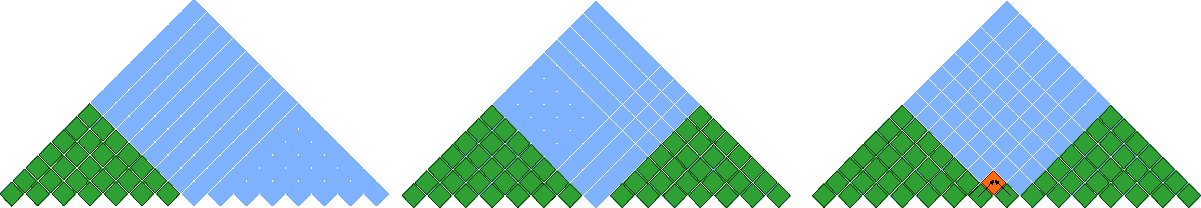
\includegraphics[width=14cm]{valsubstring.pdf}
    \caption{Количество элементов, вычисляемых в алгоритме Валианта (2 треугольные подматрицы размера $\frac{n}{2}$).}
    \label{fig5}
 \end{center}
\vspace{-8mm}
\end{figure}

Алгоритм Валианта, в отличие от модификации, не может так легко быть применен к данной задаче. В нем необходимо будет полностью вычислить, как минимум, две треугольные подматрицы размера $\frac{n}{2}$, как показано на рис.~\ref{fig5}.
Это значит, что минимальная сложность, улучшить которую без дополнительных модификаций не удастся, будет составлять $\mathcal{O}(|G|BMM(2^{p - 1})(p - 2))$.

Таким образом, в данном разделе мы показади, что алгоритм Явейн может быть эффективно применен для строк размера $s \ll n$.



\section{Реализация}

В рамках данной работы мы реализовали алгоритм Явейн несколькими способами. Мы хотели исследовать, как повлияют на производительность те или иные особенности каждой реализации. Также был реализован исходный алгоритм Валианта для сравнения и проверки эффективности модифицированного алгоритма.

\subsection{Последовательная версия}

Первая реализизация основана на использовании уже существующих библиотек. 
Языком программирования был выбран С++. Для перемножения матриц была использована библиотека для работы с плотними матрицами --- M4RI~\cite{M4RI}. 
Данная библиотека была выбрана, так как там реализован один их наиболее эффективных способов перемножения булевых матриц --- метод четырех русских~\cite{arlazarov1970economical, albrechtefficient}.  

\subsection{Параллельная версия}

Далее мы решили остановиться на использовании параллельных техник, а именно GPGPU (General-purpose computing on graphics processing units). Была создана простая реализация перемножения подматриц на языке программирования CUDA С. Использование параллельных вычислений происходит сразу на трех уровнях: само перемножение матриц (каждый элемент результирующий матрицы обрабатывается независимо), перемножение булевых матриц для каждой пары нетерминалов, которым соответствует хотя бы одно правило, и перемножение подматриц слоя для алгоритма Явейн. 


\section{Эксперименты}

В данной секции мы приводим результаты экспериментов, целью которых было исследование производительности и практической применимости алгоритма Явейн.

Эксперименты проводились на рабочей станции со следующими характеристиками:
\begin{itemize}
    \item операционная система: Linux Mint 19.1;
    \item ЦПУ: Intel i5-8250U, 1600-3400 Mhz, 4 Core(s), 8 Logical Processor(s);
    \item объем оперативной памяти: 8.0 GB;
    \item графический процессор: NVIDIA GeForce GTX 1050 MAX-Q.
\end{itemize}

Основной целью поставленных экспериментов было исследование возможностей алгоритма Явейн.
Для этого были поставлены следующие вопросы:

\begin{itemize}
    \item Сравнение алгоритмов Валианта и Явейн.
    \item Эффективность применения алгоритма Явейн к задаче поиска подстрок.
\end{itemize}

Для ответа на первый вопрос был проведен сравнительный анализ как последовательной, так и параллельной версий реализации. 

При исследовании алгоритмы были протестированы сначала на грамматике Дика для двух типов скобок~\cite{hopcroft1969formal}. Она представлена на листинге~\ref{dyck}. Данная граммматика была выбрана потому, что грамматики для описания правильных скобочных последовательностей применяются при анализе строк в биоинформатике. 

\begin{listing}
\caption{Грамматика $D2$}

\quad\quad\quad\quad\quad\quad\quad\quad\quad\quad\quad\quad s : s s  |  (s) |  [s]  |  $\epsilon$

\label{dyck}
\end{listing} 

Грамматика $D2$ переводится в нормальную форму Хомского и подается на вход алгоритму со специально сгенерированными строками различной длины (127-8191 символов). Строки составлены следующим образом: заранее создается подстрока, принадлежащая языку Дика, далее в полную строку вставляется максимально возможное количество созданных подстрок, которые можно разделить “перегородками” (терминалами, из-за которых все остальные строки, кроме вставленных, будут невыводимыми в грамматике $D2$). Строки были созданы таким образом, чтобы проверять корректность предложенного алгоритма.

Далее мы для тестирования производительности алгоритмов использовали грамматику, применяющуюся в некоторых работах по биоинформатике~\cite{bioinformatics19}. Она представлена на листинге~\ref{bio}. Грамматика $BIO$ также, как и в предыдущем случае, переводится в нормальную форму Хомского. Строки для данного эксперимента были сгенерированны случайным образом.

\begin{listing}[h]
\caption{Грамматика $BIO$}
\begin{pyglist}[]
            s1: stem<s0>
            any_str : any_smb*[2..10]
            s0: any_str | any_str stem<s0> s0
            any_smb: A | T | C | G
            stem1<s>: A s T | G s C | T s A | C s G 
            stem2<s>: stem1<stem1<s>>
            stem<s>:  
                  A stem<s> T 
                | T stem<s> A 
                | C stem<s> G 
                | G stem<s> C 
                | stem1<stem2<s>>  
\end{pyglist}
\label{bio}
\end{listing}



\subsection{Сранительный анализ}

Результаты сравнительного анализа реализаций алгоритма Валианта и Явейн представлены в таблице~\ref{tbl1} и на рис.~\ref{expPlots}. N –-- длина сгенерированной строки. Для последовательной версии алгоритма Валианта (valCPU) и Явейн (yavCPU), а также для параллельной версии --- valGPU и yavGPU соответственно, представлено время работы алгоритмов (в миллисекундах) для двух грамматик: $D2$ и $BIO$.

\begin{table*}[h]
\caption{Результаты сравнительного анализа (время в мс)}
\label{tbl1}
\centering
\small
\begin{tabular}{|| c||c|c|c|c || c|c|c|c ||} 
\hline
\multirow{2}{1em}{N} & \multicolumn{4}{c||}{Грамматика $D2$} & \multicolumn{4}{c||}{Грамматика $BIO$} \\
& valCPU & yavCPU & valGPU & yavGPU & valCPU & yavCPU & valGPU & yavGPU   \\
\hline
127 & 78 & 76 & 311 & 105 & 1345 & 1339 & 303 & 106 \\
255 & 289 & 292 & 1015 & 130 & 5408 & 5488 & 1030 & 140  \\
511 & 1212 & 1177 & 3975 & 250 & 21969 & 22347 & 4043 & 256   \\
1023 & 4858 & 4779 & 16506 & 540 & 88698 & 90318 & 16775 & 598  \\
2047 & 19613 & 19379 & 68704 & 1500 & 363324 & 374204 & 68839 & 1701  \\
4095 & 78361 & 78279 & 274832 & 4453 & 1467675 & 1480594 & 275645 & 5472 \\
8191 & 315677 & 315088 & - & 13650 & - & - & - & 18039 \\
\hline
\end{tabular}

\end{table*}

\begin{figure}[H]
\centering
\subfloat[Последовательная реализация]{
    \begin{tikzpicture}[scale=.9]
    \begin{axis}[
    legend cell align=left,
    legend pos = north west,
    xlabel = {Длина входа},
    ylabel = {Время, с},
    %ymode=log
    ]
    \addplot [color=blue, mark=triangle*] coordinates {
        (127, 0.078) (255, 0.289) (511,1.212) (1023,4.858) (2047,19.613) (4095,78.361)
    };
    \addplot [color=red, mark=*] coordinates {
        (127, 0.076) (255, 0.292) (511,1.177) (1023,4.779) (2047,19.379) (4095,78.279)
    };
    \legend{ 
        valCPU, 
        yavCPU
    };
    \end{axis}
    \end{tikzpicture}
    \label{fig:GSSedges}
}
~
\subfloat[Параллельная реализация]{
    \begin{tikzpicture}[scale=.9]
    \begin{axis}[
    legend cell align=left,
    legend pos = north west,
    xlabel = {Длина входа},
    ylabel = {Время, с},
    %ymode=log
    ]
    \addplot [color=blue, mark=triangle*] coordinates {
        (127, 0.311) (255, 1.015) (511,3.975) (1023,16.506) (2047,68.704) (4095,274.832)
    };
    \addplot [color=red, mark=*] coordinates {
        (127, 0.105) (255, 0.130) (511,0.250) (1023,0.540) (2047,1.5) (4095,4.453)
    };
    \legend{ 
        valGPU, 
        yavGPU
    };
    \end{axis}
    \end{tikzpicture}
    \label{fig:Time}
}

\caption{Результаты экспериментов с грамматикой $D2$.}
\label{expPlots}
\end{figure}


Результаты сравнительного анализа для последовательной версии показывают, что алгоритмы работают практически одинаково. Однако видно, как на последовательную реализацию влияет константа $|G|$. В нашем случае, для грамматики $D2$ количество правил при переводе в нормальную форму Хомского возрасло до 7, а для $BIO$ --- до 106. Это означает, что скорость работы алгоритмов прямо пропорциональна количеству правил грамматики. 

Параллельная версия алгоритма Валианта оказалась медленнее на грамматике $D2$, можно предположить, что это связано с большим количеством перемножений матриц небольшого размера и невозможностью их параллельной обработки. Но на больших грамматиках ($BIO$) она демонстрирует значительное улучшение производительности по сравнению с последовательной версией за счет использования параллелизма на уровне правил грамматики (то есть независимого перемножения матриц для каждой пары нетерминалов).

Лучшее время работы показывает параллельная версия алгоритма Явейн. Это связано с тем, что параллелизм используется сразу на трех уровнях, как было замечено в предыдущем разделе. 

\subsection{Применимость к задаче поиска подстрок}

Для алгоритма Явейн была изменена функция $main()$: теперь она принимает дополнительный аргумент s --- длину максимальной искомой подстроки и вычисляет только те слои, которые содержат в себе нужные подстроки, как было показано в разделе 4.

Результаты работы адаптированного к задаче поиска подстрок алгоритма Явейн представлены в таблице~\ref{tbl3}. N – длина сгенерированной строки. Для последовательной (adpСPU) и параллельной (adpGPU) версии реализации представлено время работы в миллисекундах.

\begin{table*}[h]

\begin{center}
\caption{Результаты работы алгоритма Явейн для задачи поиска подстрок (время в мс)}
\label{tbl3}
    \begin{tabular}{ ||c||c||c|c|| } 
    \hline
    s & N & adpCPU &  adpGPU \\
    \hline
    \multirow{4}{2em}{250} & 1023 & 2996 & 242 \\ 
    & 2047 & 6647 & 255\\ 
    & 4095 & 13825 & 320\\ 
    & 8191 & 28904 & 456\\ 
    \hline
    \multirow{3}{2em}{510} & 2047 & 12178 & 583\\
    & 4095 & 26576 & 653\\
    & 8191 & 56703 & 884\\ 
    \hline
    \multirow{2}{2em}{1020} & 4095 & 48314 & 1590 \\
    & 8191 & 108382 & 1953\\ 
    \hline
    2040 & 4095 & 197324 & 5100\\ 
    \hline
    \end{tabular}
\end{center}

\end{table*}


Результаты второго эксперимента показывают, что адаптированная версия алгоритма Явейн может быть эффективно применена к задаче поиска подстрок: она корректно находит все выводимые подстроки в строке и работает существенно быстрее алгоритма Валианта (см. таблицу~\ref{tbl1}), который будет совершать большое количество лишних вычислений из-за сложности его преждевременной остановки.

Таким образом, проведенные эксперименты показали практическую применимость алгоритма Явейн, возможность его существенного ускорения за счет использования параллельных вычислений и адаптации к задаче поиска подстрок.

\section{Заключение}
В данной работе были получены следующие результаты.

\begin{itemize}
	\item Изучен алгоритм Явейн, являющийся модификацией алгоритма Валианта, основной особенностью которого является возможность разбиения матрицы на слои, что упрощает разработку параллельной версии алгоритма и применимость к задаче поиска подстрок.  
	\item Проведен анализ, который показал, что алгоритм Явейн лучше применим к задаче поиска подстрок, чем оригинальная версия алгоритма.
	\item Доказана корректность алгоритма Явейн и дана оценка вычислительной сложности, которая составляет $\mathcal{O}(BMM(n)log(n))$.
	\item Реализованы последовательная и параллельная версии алгоритмов. Исходный код доступен в репозитории: https://github.com/SusaninaJulia/PBMM.
	\item Проведено экспериментальное исследование алгоритма, показавшее эффективность модификации: последовательные версии алгоритмов Валианта и Явейн работают одинаково; параллельная версия алгоритма Явейн показывает значительный прирост производительности на строка большей длины; показана эффективность применения алгоритма Явейн к задаче поиска подстрок.
\end{itemize}

Кроме того, мы можем определить несколько направлений будущих исследований. 
Например, оптимизация алгоритмов перемножения матриц за счет использования разделяемой памяти.
Еще планируется расширить алгоритм Явейн для других классов грамматик, которые применяются в биоинформатике: конъюнктивных и булевых.
Также, открытым остается вопрос, можно ли как-либо изменить порядок перемножения подматриц, чтобы полностью избавить алгоритм от рекурсивных вызовов.

\setmonofont[Mapping=tex-text]{CMU Typewriter Text}
\bibliographystyle{ugost2008ls}
\bibliography{references}

\end{document}